%%%%%%%%%%%%%%%%%%%%%%%%%%%%%%%%%%%%%%%%%
% CN2 Labreport template
%
% License:
% CC BY-NC-SA 3.0 (http://creativecommons.org/licenses/by-nc-sa/3.0/)
%
%%%%%%%%%%%%%%%%%%%%%%%%%%%%%%%%%%%%%%%%%

\documentclass[parskip=full]{scrartcl}

\usepackage{siunitx}  % Provides the \SI{}{} command for typesetting SI units
\usepackage{graphicx} % Required for the inclusion of images
\usepackage{booktabs} % nicer tables
\usepackage[noabbrev]{cleveref} % automatic references
\usepackage{listings} % typeset code
\usepackage[backend=biber]{biblatex}
\addbibresource{referenzen.bib}

\crefname{lstlisting}{listing}{listings} % for referencing code
\Crefname{lstlisting}{Listing}{Listings} % for referencing code

\usepackage[headsepline]{scrlayer-scrpage} % header
\ohead{Group 06} % right part of header
\ihead{Assignment 4} % left part of header

\lstset{basicstyle=\ttfamily} % monospaced font in listing

% Automata 
\usepackage{pgfplots}
\usetikzlibrary{automata,arrows,positioning} 

%----------------------------------------------------------------------------------------
%	DOCUMENT INFORMATION
%----------------------------------------------------------------------------------------

\begin{document}
\begin{titlepage}
    \centering
    \vspace*{2cm}
    {\Huge \textbf{Communication Networks 2}}\\
    SS 2021\\
    \vspace*{1cm}
    {\Large Assignment 4}
    \\\vspace*{3cm}
    {\Large \textbf{Group 06}}\\
    \vspace*{1cm}
    {\large 
        \begin{tabular}{l c c}
            Name & Mat.Nummer \\ \hline
            Paul Kloker & 12034928 \\
            Juan Aramis Oposich & 11701238
        \end{tabular}
    }
    \\\vspace*{7cm}
    \today
\end{titlepage}

%----------------------------------------------------------------------------------------
%	SECTION 1
%----------------------------------------------------------------------------------------
\section{Task description and setup} \label{sec:task}
The task of the last assignment is to model a network in NS-3, which is an open source network simulator, according to the following network diagram (\cref{fig:2a}).
Furthermore, a 10 seconds long simulation with a ping measurement from node 1 to node 3 shall be done and the generated measurement data discussed.
\begin{figure}[!h]
	\centering
	\begin{tikzpicture}[ >=stealth', auto, semithick, node distance=6cm]
	\tikzstyle{every state}=[fill=white,draw=black,thick,text=black,scale=1]
	\node[state]    (0)               {$1$};
	\node[state]    (1)[right of=0]   {$2$};
	\node[state]    (2)[ right of=1]  {$3$};
	\path
	(0)	edge[above left] 	    	node{$10.0.120.2\ \ \ \ $}		(1)
	(0)	edge[above right] 	    	node{$\ \ \ \ 10.0.120.1$}		(1)
	(0)	edge[below] 	    		node{$PointToPoint$}				(1)
	(1)	edge[above left] 	    	node{$10.0.248.1\ \ \ \ $}		(2)
	(1)	edge[above right] 	    	node{$\ \ \ \ 10.0.248.2$}		(2)
	(1)	edge[below] 	    		node{$CSMA$}				(2);
	
	\end{tikzpicture}
	\caption{Network topology}
	\label{fig:2a}
\end{figure}

For this the latest version of NS-3 was downloaded form \verb|https://www.nsmam.org| and build with the command \verb|$ ./bulid.py|. 


%----------------------------------------------------------------------------------------
%	SECTION 2
%----------------------------------------------------------------------------------------
\section{NS3 Model} \label{sec:procedure}
NS-3 models are C++ based and consist out of network nodes, network devices, communication channels and applications.
Most of the code is based on the second tutorial in the example folder.
Listing \ref{lst:creation} shows the creation of the topology
Because our system consists out of one PointToPoint connection and one Carrier Sense Multiple Access (CSMA) network, different kind of nodes were created and the given channel attributes were set by using the helper objects.
To finish the topology creation helper objects were used to install the network devices and a IP stack for every node.

\begin{lstlisting}[language=c++, frame=single, captionpos=b, caption={Topology creation}, label=lst:creation]
//P2P
NodeContainer p2pNodes;
p2pNodes.Create (2);

PointToPointHelper pointToPoint;
pointToPoint.SetDeviceAttribute ("DataRate", 
                                  StringValue ("11Mbps"));
pointToPoint.SetChannelAttribute ("Delay", 
                                   StringValue ("80ms"));
                                   
NetDeviceContainer p2pDevices;
p2pDevices = pointToPoint.Install (p2pNodes);

//CSMA
NodeContainer csmaNodes;
csmaNodes.Add (p2pNodes.Get (0));
csmaNodes.Create (1);

CsmaHelper csma;
csma.SetChannelAttribute ("DataRate", 
                           StringValue ("70Mbps"));
csma.SetChannelAttribute ("Delay", 
                           TimeValue (MicroSeconds (1000)));
                           
NetDeviceContainer csmaDevices;
csmaDevices = csma.Install (csmaNodes);

InternetStackHelper stack;the
stack.Install (p2pNodes.Get (1));
stack.Install (csmaNodes);
\end{lstlisting}


\begin{table}[hb]
	\centering
	\begin{tabular}{lll}
		\toprule
		\textbf{Node No.} & \textbf{NS-3 Node Container Element} & \textbf{IP Address}\\ \midrule
		1 & p2pNodes.Get(1) & 10.0.120.2 \\
		2 & p2pNodes.Get(0) & 10.0.120.1 \\
		2 & csmaNodes.Get(0) & 10.0.248.1 \\
		3 & csmaNodes.Get(1) & 10.0.248.2 \\
		\bottomrule
	\end{tabular}
	\caption{Nodes and the according NS-3 node container element}
	\label{tab:Nodes}
\end{table}

To create a routing table with the \verb|Ipv4GlobalRoutingHelper|, both subnets first got the right address space assigned to them (see \ref{lst:address}).

\begin{lstlisting}[language=c++, frame=single, captionpos=b, caption={IP address assignment and routing table creation}, label=lst:address]
Ipv4AddressHelper address;
address.SetBase ("10.0.120.0", "255.255.255.0");
Ipv4InterfaceContainer p2pInterfaces;
p2pInterfaces = address.Assign (p2pDevices);

address.SetBase ("10.0.248.0", "255.255.255.0");
Ipv4InterfaceContainer csmaInterfaces;
csmaInterfaces = address.Assign (csmaDevices);

Ipv4GlobalRoutingHelper::PopulateRoutingTables ();
\end{lstlisting}

Listing \ref{lst:ping} shows how the ping to the third node was created and installed on the first node. 
The attribute \verb|Verbose| was set to true to create a ping-style output. 
The payload was set to 1024 bytes and the interval between the ping messages to 0.2 Seconds.
The last two lines of \cref{lst:ping} define how long the ping application will run during the simulation

\begin{lstlisting}[language=c++, frame=single , captionpos=b, label=lst:ping]
V4PingHelper ping = V4PingHelper (
		    csmaInterfaces.GetAddress (1));
ping.SetAttribute ("Verbose", BooleanValue (true));
ping.SetAttribute ("Size", UintegerValue(1024));
ping.SetAttribute ("Interval", TimeValue(Seconds(0.2)));
ApplicationContainer apps = ping.Install (p2pNodes.Get (1));
apps.Start (Seconds (1.0));
apps.Stop (Seconds (10.0));
}
\end{lstlisting}

Before the simulation was invoked the stop time was specified and packet capturing was enabled for all P2P and CSMA nodes (see \cref{lst:simulation}).

\begin{lstlisting}[language=c++, frame=single , captionpos=b, caption={pcap and simulation start}, label=lst:simulation]
csma.EnablePcapAll("assignment4", true);
pointToPoint.EnablePcapAll ("assignment4", true);

Simulator::Stop (Seconds (10.0));
Simulator::Run ();
Simulator::Destroy ();
}
\end{lstlisting}

The code was then compiled and execute with \verb|waf|. This created the ping measurement and pcap data which will be discussed in the next section. 

\section{Data analysis and comparison} \label{sec:data}


\begin{table}[hb]
	\centering
	\begin{tabular}{ll}
		\toprule
		\textbf{End-to-End delay} & \textbf{User experience} \\ \midrule
			$T_{EE} < 150$ & acceptable for all users \\
			$150 < T_{EE} < 300$ & noticeable quality degradation, but still acceptable for most users\\
			$T_{EE} \geq 300$ & not acceptable\\
			\bottomrule
		\end{tabular}
		\caption{Delay to user experience}
		\label{tab:delayEnd2End}
	\end{table}

\begin{figure}[!ht]
	\centering % centering figure 
	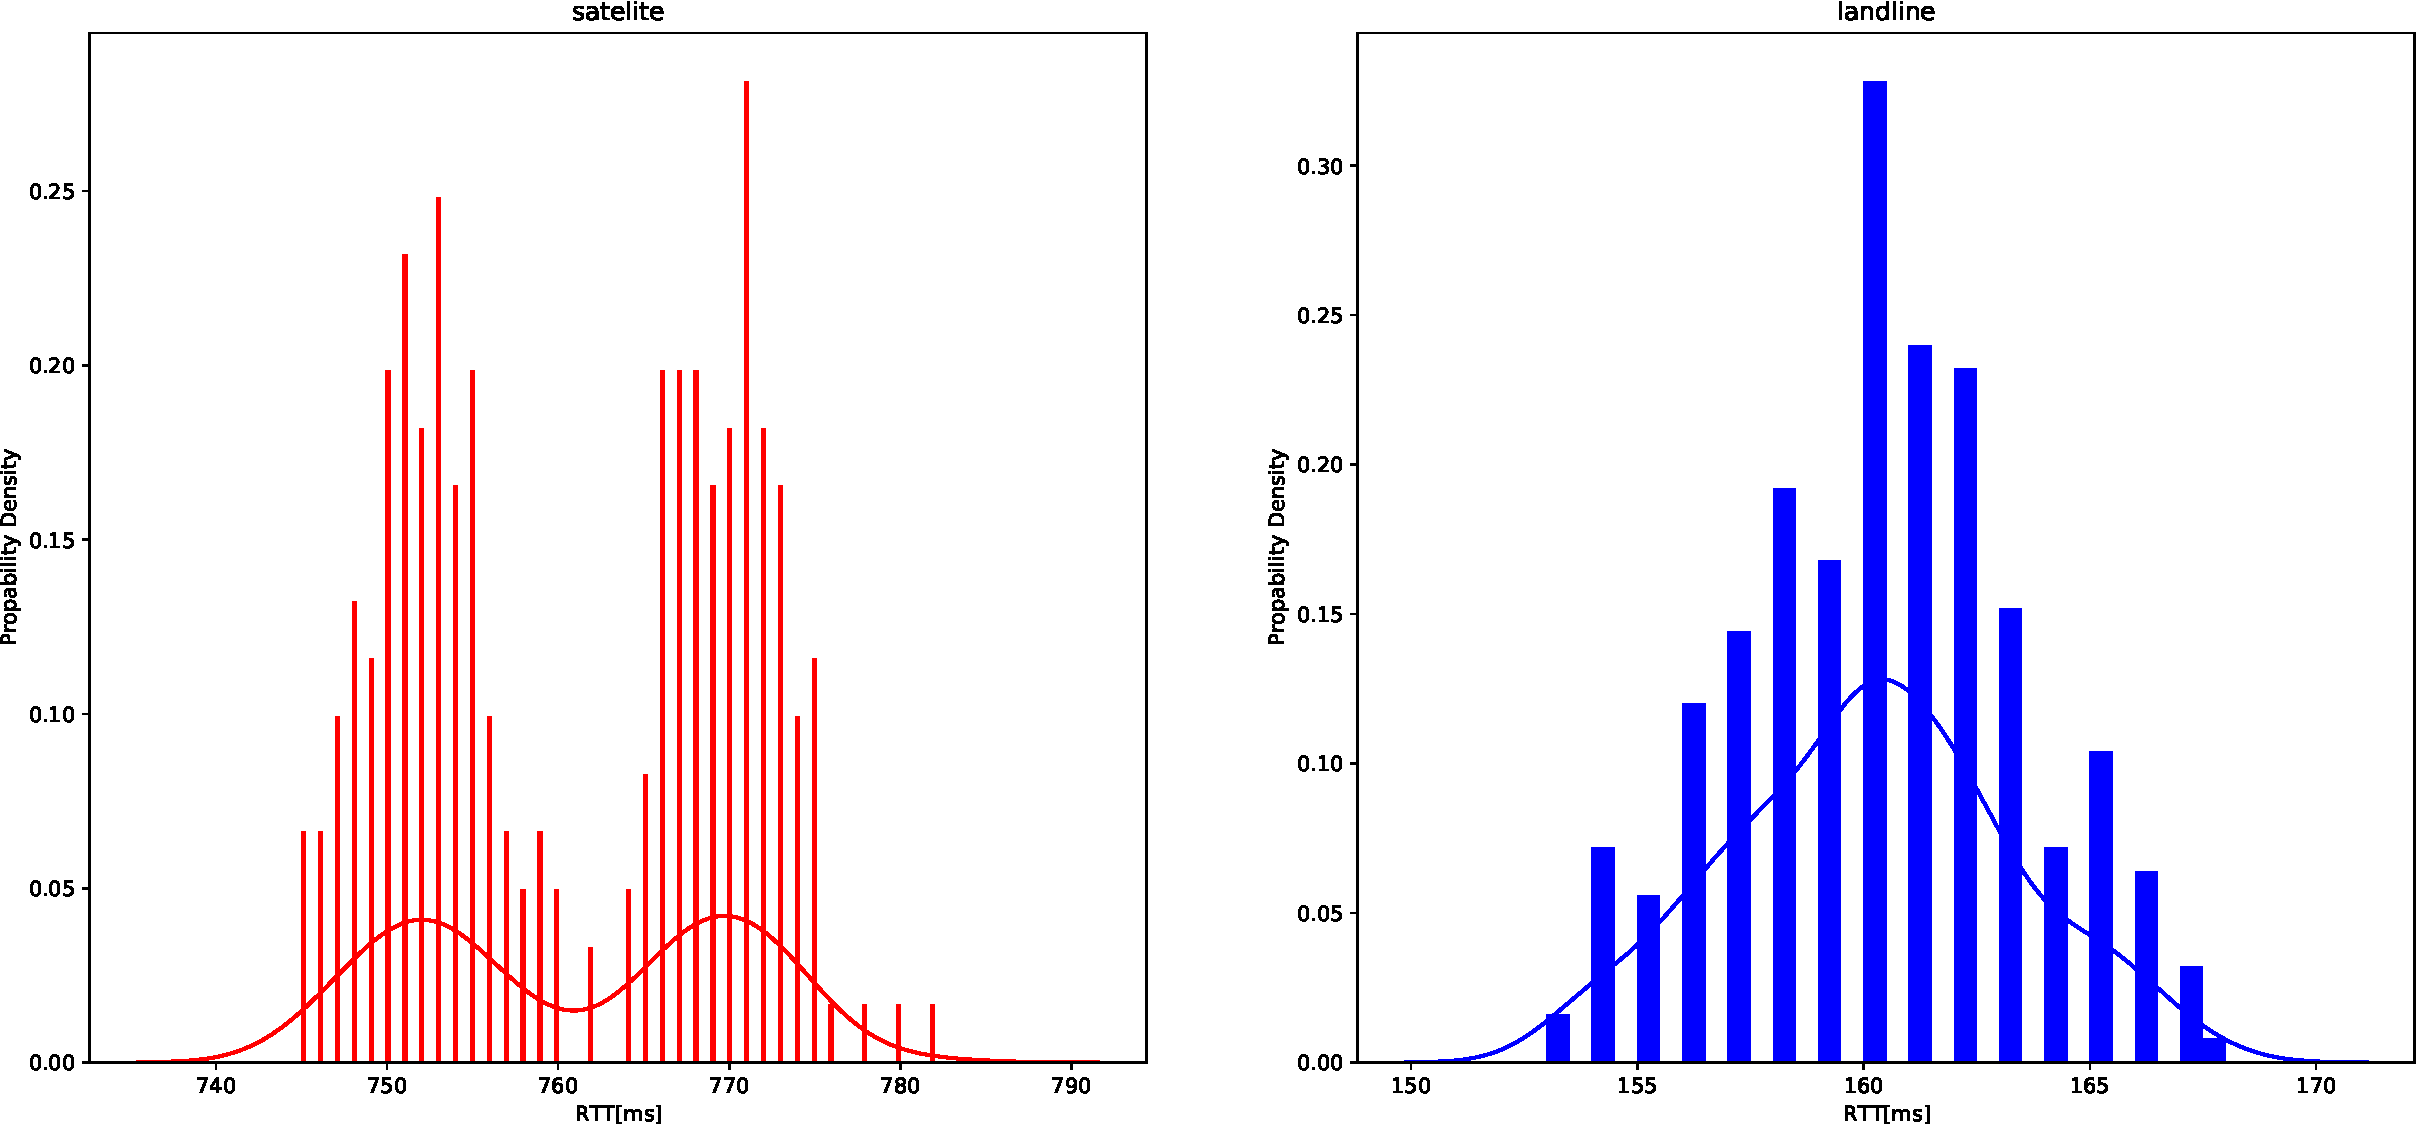
\includegraphics[width=\textwidth]{images/oneWayDelay.pdf} % importing figure
	\caption{Propobility density of one way delay} 
	\label{fig:one-way-delay} % labeling to refer it inside the text
\end{figure}


%----------------------------------------------------------------------------------------
%	SECTION 3
%----------------------------------------------------------------------------------------

\section{Conclusion}



%----------------------------------------------------------------------------------------
%	SECTION X
%---------------------------------------------------------------------------------------

\printbibliography

\end{document}
